
All used languages have functional and concurrent built-in features, with the first ones supporting the second ones. Erlang and Scala’s implementations are based in the actor pattern for doing parallel computation. Clojure on the other hand works with the agent concept, a similar model with simplified ways of reading the involved information.

To communicate modules we used language’s dependent (and different) data types.
The message's structure was tuples for Erlang and Scala, and for agents it was necessary to encapsulate functions on protocols (Clojure variants of Java interfaces). For sharing individuals (the pool) we used functionals consult/modification data structures: hash-like for Scala/Clojure and the {\em ets} module in Erlang’s case. The data was encoded with compound data structures: lists, vectors, tuples, records, etc. The Table \ref{tb:res:comp} summarizes the differences between the languages.

\begin{table}
  \caption{Language concept used for each pGA component.}\label{tb:res:comp}
  \centering
  \begin{tabular}{|p{2.2cm}|>{\centering}p{1.6cm}|>{\centering}p{1.6cm}|>{\centering}p{1.8cm}|}
    \hline
     & \textbf{Erlang} & \textbf{Scala} & \textbf{Clojure} \tabularnewline
    \hline
    Parallel execution unit & actor & actor & agent \tabularnewline
    \hline
    Communication (messages) & tuple & tuple & function (protocol) \tabularnewline
    \hline
    pool & \emph{ets} & HashMap & hash-map \tabularnewline
    \hline
    DS chromosome & list & list & vector \tabularnewline
    \hline
    DS population & list & list & lazy list \tabularnewline
    \hline
    Compound data & tuple & tuple/object & record/vector \tabularnewline
    \hline
    Runtime environment & Erlang VM & Java VM & Java VM \tabularnewline
    \hline
  \end{tabular}

\end{table}


\simpleEntry{Results}

The design was tested with a population of 1024 individuals on each island (two islands were used), doing 5000 evaluations on a dual-core (4 threads) laptop  i7-3520M with Windows 8 and 16 Gb of RAM. In order to find the better combinations of evaluators/reproducers, several of them were tested for each technology (evaluators = $1..30$ and reproducers = $1..10$). In every combination the number of evaluators is greater than the reproducers because the fitness function is more computational intensive than the reproduction execution. 10 runs were used for each combination and then the times with more dispersion were deleted until the standard deviation (SD) remained below the 5 \%.

For a \emph{speedup} analysis, using the ideas presented in \cite{Alba02parallelevolutionary},  a sequential implementation with the same data structures and operator's implementations was made. Speedup is the ratio between $E[T_1]$ (sequential implementation average time) and $E[T_m]$ (parallel implementation average time in $m$ processors), the expected value is $m=4$ in this case (the number of logical processors in the used hardware).

\begin{table}
  \caption{Experiment results for the minimum parallel time of all combinations tested.}\label{tb:resAll}
  \centering
\begin{tabular}{|>{\centering}p{.85cm}|>{\centering}p{1.4cm}|
>{\centering}p{1.4cm}|>{\centering}p{.9cm}|>{\centering}p{1cm}|
>{\centering}p{.8cm}|>{\centering}p{.45cm}|}
  \hline
  \textbf{Language} & \textbf{Parallel time $\pm$ SD (ms)} & \textbf{Workers combination} & \textbf{Sequential time (ms)} & \textbf{Relative speedup} & \textbf{Speedup}\tabularnewline
  \hline
  Erlang & 2920.40 $\pm$ 126 & 25 evaluators, 1 reproducer & 8143.3 & 2.78 & 0.55 \tabularnewline
  \hline
  Clojure & 1734.66 $\pm$ 28.32 & 10 evaluators, 1 reproducer & 3340.22 & 1.92 & 0.92 \tabularnewline
  \hline
  Scala & 563 $\pm$ 24.32 & 6 evaluators, 1 reproducer & 1651.8 & 2.86 & 2.86 \tabularnewline
  \hline
\end{tabular}
\end{table}

The results shown in Table \ref{tb:resAll} indicate for each language the best time for the parallel implementation, the combination of evaluators/reproducers in which the parallel variant was obtained, the time for the sequential implementation, a relative speedup (calculated in relation to his sequential time) and the speedup (relative to the best sequential time, Scala's in this case). Each worker (evaluators and reproducers) is a unit of execution, and in the used hardware only 4 units (at most) can run at the same time.

Figure 1 shows the running times when one reproducer is used with a variant number of evaluators;  Figure 2 shows the same but for two reproducers. In both cases the overall behaviour of Scala is better. The computation complexity of the evaluation function is greater than the reproduction phase and this is why the results when one reproducer was used are better than when two reproducers were used.


\begin{small}
\begin{itemize}
\item[] \textbf{Fig. 1.} Parallel running times for one reproducer and 0..30 evaluators of hybrid pGAs implementation in Erlang, Scala and Clojure.
    
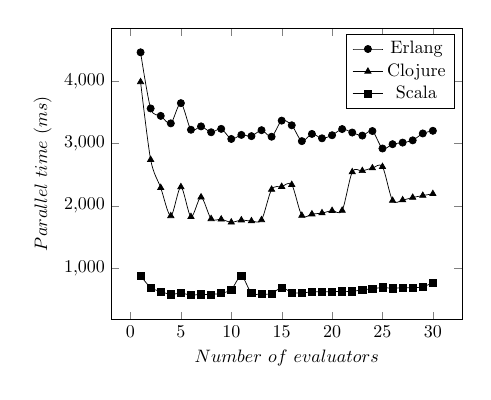
\begin{tikzpicture}[thick, scale=0.65]

  \begin{axis}[
         xlabel=$Number \hspace{.12cm} of \hspace{.12cm} evaluators$,
         ylabel=$Parallel \hspace{.12cm} time \hspace{.12cm} (ms)$
         ]
     \addplot[smooth,mark=*]  plot coordinates{
(1,4466.6)
(2,3564.222222222222)
(3,3444.6666666666665)
(4,3324.5555555555557)
(5,3649.6)
(6,3221.7)
(7,3275.9)
(8,3181.3)
(9,3236.0)
(10,3073.5555555555557)
(11,3139.0)
(12,3119.1111111111113)
(13,3214.9)
(14,3109.5555555555557)
(15,3368.3)
(16,3293.7)
(17,3039.1)
(18,3154.7)
(19,3084.1)
(20,3133.6666666666665)
(21,3232.9)
(22,3177.1111111111113)
(23,3128.0)
(24,3201.3333333333335)
(25,2920.4)
(26,2989.5555555555557)
(27,3015.4)
(28,3051.4444444444443)
(29,3162.3)
(30,3204.7)
     };
     \addlegendentry{Erlang}

     \addplot[smooth,mark=triangle*]
         plot coordinates{
(1,3990.75)
(2,2740.777777777778)
(3,2289.1111111111113)
(4,1837.111111111111)
(5,2302.5555555555557)
(6,1822.6666666666667)
(7,2138.6666666666665)
(8,1789.5)
(9,1782.3333333333333)
(10,1734.6666666666667)
(11,1768.888888888889)
(12,1754.7777777777778)
(13,1772.0)
(14,2261.1111111111113)
(15,2307.8888888888887)
(16,2338.4444444444443)
(17,1842.3333333333333)
(18,1865.7777777777778)
(19,1883.4444444444443)
(20,1920.7777777777778)
(21,1923.5)
(22,2542.1111111111113)
(23,2561.6666666666665)
(24,2605.5555555555557)
(25,2627.0)
(26,2083.0)
(27,2091.8888888888887)
(28,2132.222222222222)
(29,2163.777777777778)
(30,2192.1111111111113)
         };
     \addlegendentry{Clojure}


     \addplot[smooth,mark=square*]
         plot coordinates{
(1,876.6666666666666)
(2,683.7777777777778)
(3,622.2857142857143)
(4,575.2222222222222)
(5,596.0)
(6,563.0)
(7,576.2222222222222)
(8,574.0)
(9,595.1111111111111)
(10,651.8888888888889)
(11,871.6666666666666)
(12,595.3333333333334)
(13,582.25)
(14,586.8888888888889)
(15,684.8888888888889)
(16,605.0)
(17,600.625)
(18,614.0)
(19,618.2222222222222)
(20,616.7777777777778)
(21,625.2222222222222)
(22,622.6666666666666)
(23,649.7777777777778)
(24,664.1111111111111)
(25,686.625)
(26,672.4444444444445)
(27,684.7777777777778)
(28,681.625)
(29,698.0)
(30,760.7142857142857)
         };
     \addlegendentry{Scala}

  \end{axis}

\end{tikzpicture}



\item[] \textbf{Fig. 2.} Parallel running times for two reproducers and 0..30 evaluators of hybrid pGAs implementation in Erlang, Scala and Clojure.
    
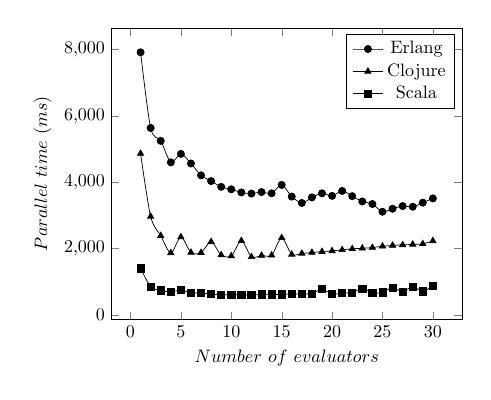
\begin{tikzpicture}[thick, scale=0.65]

  \begin{axis}[
         xlabel=$Number \hspace{.12cm} of \hspace{.12cm} evaluators$,
         ylabel=$Parallel \hspace{.12cm} time \hspace{.12cm} (ms)$
         ]
     \addplot[smooth,mark=*]  plot coordinates{
(1,7919.428571428572)
(2,5638.0)
(3,5249.75)
(4,4601.5)
(5,4856.714285714285)
(6,4567.285714285715)
(7,4208.333333333333)
(8,4036.0)
(9,3862.777777777778)
(10,3788.3)
(11,3693.6)
(12,3659.2)
(13,3705.1111111111113)
(14,3667.0)
(15,3920.4)
(16,3568.2)
(17,3376.75)
(18,3544.7)
(19,3668.222222222222)
(20,3589.4)
(21,3739.222222222222)
(22,3580.9)
(23,3421.6)
(24,3345.222222222222)
(25,3110.8)
(26,3202.4)
(27,3282.1)
(28,3262.0)
(29,3385.4)
(30,3513.777777777778)
     };
     \addlegendentry{Erlang}

     \addplot[smooth,mark=triangle*]
         plot coordinates{
         (1,4866.5)
(2,2970.0)
(3,2389.5555555555557)
(4,1870.5555555555557)
(5,2347.1111111111113)
(6,1882.888888888889)
(7,1878.111111111111)
(8,2206.1111111111113)
(9,1808.4444444444443)
(10,1777.3333333333333)
(11,2238.1111111111113)
(12,1752.3333333333333)
(13,1791.888888888889)
(14,1798.888888888889)
(15,2324.777777777778)
(16,1825.7777777777778)
(17,1854.5555555555557)
(18,1881.5555555555557)
(19,1908.6666666666667)
(20,1931.5555555555557)
(21,1962.888888888889)
(22,1993.6666666666667)
(23,2010.111111111111)
(24,2030.5555555555557)
(25,2071.0)
(26,2094.3333333333335)
(27,2112.8888888888887)
(28,2126.4444444444443)
(29,2144.5555555555557)
(30,2233.222222222222)
         };
     \addlegendentry{Clojure}


     \addplot[smooth,mark=square*]
         plot coordinates{
(1,1406.8333333333333)
(2,854.5714285714286)
(3,741.0)
(4,694.75)
(5,752.2)
(6,660.1111111111111)
(7,663.4285714285714)
(8,626.5)
(9,605.375)
(10,609.125)
(11,602.7777777777778)
(12,596.1428571428571)
(13,620.8888888888889)
(14,619.7777777777778)
(15,619.0)
(16,634.2222222222222)
(17,631.8888888888889)
(18,641.8888888888889)
(19,775.5555555555555)
(20,630.625)
(21,656.6666666666666)
(22,672.7777777777778)
(23,796.2222222222222)
(24,671.1111111111111)
(25,679.3333333333334)
(26,825.8888888888889)
(27,696.2222222222222)
(28,854.5)
(29,711.0)
(30,882.6666666666666)
         };
     \addlegendentry{Scala}

  \end{axis}

\end{tikzpicture}



\end{itemize}
\end{small}


% \begin{multicols}{2}
% \begin{small}
% \begin{itemize}
% \item[] \textbf{Fig. 3.} Number of evaluators with best results for one reproducer.
%     
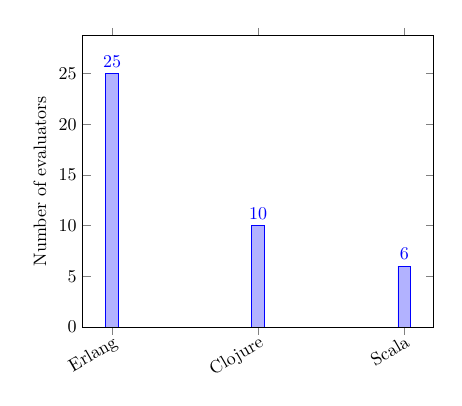
\begin{tikzpicture}[thick, scale=0.65]
  \begin{axis}[ybar,
    bar width=0.25cm,
    ymin=0,
    enlarge y limits={upper,value=0.15},
    legend style={at={(0.5,-0.25)},
    anchor=north,legend columns=-1},
    ylabel={Number of evaluators},
    symbolic x coords={Erlang, Clojure, Scala},
    xtick=data,
    xticklabel style={
        inner sep=0pt,
        anchor=north east,
        rotate=30
    },
    nodes near coords={\pgfmathprintnumber[fixed,precision=0]{\pgfplotspointmeta}},
    ]
    \addplot coordinates {(Erlang,25) (Clojure,10) (Scala,6)};
  \end{axis}
\end{tikzpicture}

% \columnbreak
% \item[] \textbf{Fig. 4.} Number of evaluators with best results for two reproducers.
%     
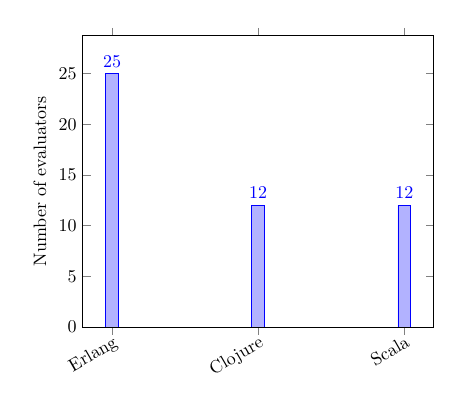
\begin{tikzpicture}[thick, scale=0.65]
  \begin{axis}[ybar,
    bar width=0.25cm,
    ymin=0,
    enlarge y limits={upper,value=0.15},
    legend style={at={(0.5,-0.25)},
    anchor=north,legend columns=-1},
    ylabel={Number of evaluators},
    symbolic x coords={Erlang, Clojure, Scala},
    xtick=data,
    xticklabel style={
        inner sep=0pt,
        anchor=north east,
        rotate=30
    },
    nodes near coords={\pgfmathprintnumber[fixed,precision=0]{\pgfplotspointmeta}},
    ]
    \addplot coordinates {(Erlang,25) (Clojure,12) (Scala,12)};
  \end{axis}
\end{tikzpicture}

% \end{itemize}
% \end{small}
% \end{multicols}

%\begin{small}
%\begin{itemize}
%\item[] \textbf{Fig. 3.} Parallel time for 25 evaluators (Erlang's best case).
%    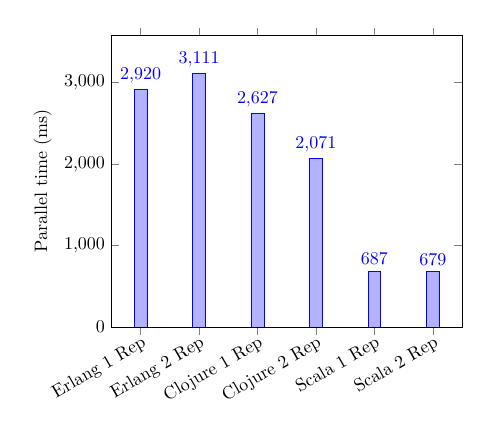
\begin{tikzpicture}[thick, scale=0.65]
  \begin{axis}[ybar,
    bar width=0.25cm,
    ymin=0,
    enlarge y limits={upper,value=0.15},
    legend style={at={(0.5,-0.25)},
    anchor=north,legend columns=-1},
    ylabel={Parallel time (ms)},
    symbolic x coords={Erlang 1 Rep, Erlang 2 Rep, Clojure 1 Rep, Clojure 2 Rep, Scala 1 Rep, Scala 2 Rep},
    xtick=data,
    xticklabel style={
        inner sep=0pt,
        anchor=north east,
        rotate=30
    },
    nodes near coords={\pgfmathprintnumber[fixed,precision=0]{\pgfplotspointmeta}},
    ]
    \addplot coordinates {(Erlang 1 Rep,2920.4) (Erlang 2 Rep,3110.8) (Clojure 1 Rep,2627) (Clojure 2 Rep,2071) (Scala 1 Rep,686.625) (Scala 2 Rep,679.3333333)};
  \end{axis}
\end{tikzpicture}
%
%
%\item[] \textbf{Fig. 4.} Parallel time for 10 evaluators (Clojure's best case).
%    
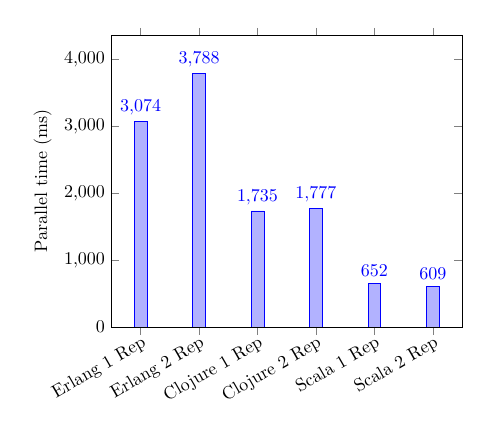
\begin{tikzpicture}[thick, scale=0.65]
  \begin{axis}[ybar,
    bar width=0.25cm,
    ymin=0,
    enlarge y limits={upper,value=0.15},
    legend style={at={(0.5,-0.25)},
    anchor=north,legend columns=-1},
    ylabel={Parallel time (ms)},
    symbolic x coords={Erlang 1 Rep, Erlang 2 Rep, Clojure 1 Rep, Clojure 2 Rep, Scala 1 Rep, Scala 2 Rep},
    xtick=data,
    xticklabel style={
        inner sep=0pt,
        anchor=north east,
        rotate=30
    },
    nodes near coords={\pgfmathprintnumber[fixed,precision=0]{\pgfplotspointmeta}},
    ]
    \addplot coordinates {(Erlang 1 Rep,3073.555556) (Erlang 2 Rep,3788.3) (Clojure 1 Rep,1734.666667) (Clojure 2 Rep,1777.333333) (Scala 1 Rep,651.8888889) (Scala 2 Rep,609.125)};
  \end{axis}
\end{tikzpicture}
%
%\end{itemize}
%\end{small}

Figures 1 and 2 show that the three languages have a good concurrent behaviour: the overhead of managing more logical execution units than the available physical ones did not show any impact on the execution time of the algorithm, even when that number gradually increases.

%\setcounter{figure}{4}
%
%\begin{figure}
%\caption{Parallel time for 6 evaluators (Scala's best case).}
%\centering
%    
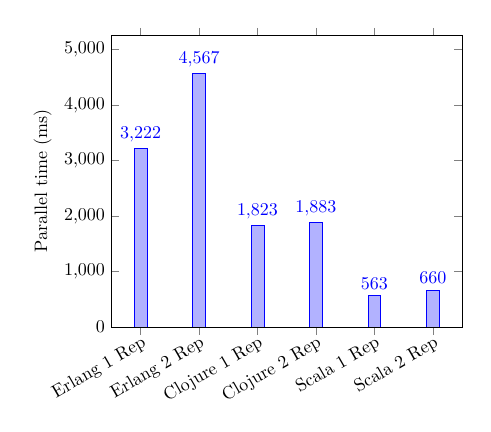
\begin{tikzpicture}[thick, scale=0.65]
  \begin{axis}[ybar,
    bar width=0.25cm,
    ymin=0,
    enlarge y limits={upper,value=0.15},
    legend style={at={(0.5,-0.25)},
    anchor=north,legend columns=-1},
    ylabel={Parallel time (ms)},
    symbolic x coords={Erlang 1 Rep, Erlang 2 Rep, Clojure 1 Rep, Clojure 2 Rep, Scala 1 Rep, Scala 2 Rep},
    xtick=data,
    xticklabel style={
        inner sep=0pt,
        anchor=north east,
        rotate=30
    },
    nodes near coords={\pgfmathprintnumber[fixed,precision=0]{\pgfplotspointmeta}},
    ]
    \addplot coordinates {(Erlang 1 Rep,3221.7) (Erlang 2 Rep,4567.285714) (Clojure 1 Rep,1822.666667) (Clojure 2 Rep,1882.888889) (Scala 1 Rep,563) (Scala 2 Rep,660.1111111)};
  \end{axis}
\end{tikzpicture}
%\end{figure}

The Scala implementation is smoother in its results in contrast with
Clojure where many peaks were obtained. % Y habría que ver por qué - JJ
These two languages use the JVM and the same random library, however there are clear differences in their concurrent models. The results for Scala and Clojure are better with a small number of units of execution: when the number of evaluators grows the efficiency of the algorithm falls. In this sense Erlang have a non-typical behaviour, improving up to 25 evaluators, and then the speed begins to decrease.

Erlang is the language with the worst execution time; but its runtime, in the best case, is able to schedule 52 units of execution (far more than the others). The Erlang processes are scheduled using SMP whith one scheduler per core. Each process is allowed to run until it is paused to wait for input (a message from some other processes) or until it has executed a maximum fixed number of reductions (each VM instruction has associated a number of reductions). This unique way of scheduling processes yields these particular results and will be better used in next studies. Also the speedup obtained in relationship with his sequential time is very good. These two facts point to a possible good scalability.

Clojure's performance is medium, with a speedup close to $1$. The {\em send} function was always used to compute the expression by the agents therefore a hardware dependent pool of treats was used.

Scala is the language with best results, even when its runtime is the same of Clojure's. It has a particular model of concurrency (actors on a {\em event-based} dispatcher supported on the Java JSR166 fork-join pool); and of computation (its balance between mutable and immutable state), allowing the best behaviour of the concurrent algorithm. Again is important to note the quality of the concurrent abstractions made by all these technologies in which the number of logical units of executions is greater than the number of the physical ones.

